\section{Person Map Location}

In this section, the task was to use linear algebra to map a person walk from video source taken at an angle to the overview map of the ITU. We have been given a video file where a person can be seen walking in the atrium of the IT University of Copenhagen, trace data that represents the person's position in each frame in the video, and an overview map of the ITU. We have also had a tool at our disposal that allowed us to obtain the homography matrix from the video to the map. 

We started by obtaining the homography matrix. We have specified four points in a frame of the provided video, and then we have tried to select the exact same points on the overview map. All of the four points had to lay on a plane, because a homography matrix describes the relation between two views of the same plane. We also need at least four points, because otherwise (e.g with three points) we would only be able to describe an affine transformation, not a projection. It is important to note, that since the entire video sequence of the walk is taken from a stationary camera (i.e the camera does not move during the exposition), and because the overview map of ITU is also not changing, it is sufficient to calculate the homogaphy once for the entire sequence. Otherwise we would need to recalculate it for each frame when the relative position of the camera and the ground plane has changed.

\begin{figure}[h!]
	\centering
	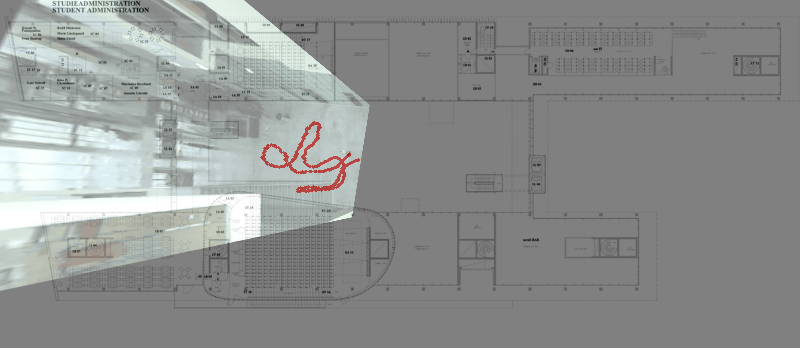
\includegraphics[width=\textwidth]{Handin2/images/trace_map.png}
	\caption{Trace Map}
	\label{fig:trace}
\end{figure}

Using the obtained homography matrix we have been then able to project the video image onto the overview map of ITU which can be seen in the Figure \ref{fig:trace}. Using the trace data provided we have then been able to position the person in the overview map. We have taken the center point of the bottom edge of the rectangle describing the person's legs. This point should always be on the ground and therefore should guarantee the best approximation of the person's actual position (as opposed to the head for example, which would form a triangle between head, legs and a point defined by camera angle further away from the camera on the floor, yielding an inaccuracy of around the person's height at this camera angle).

\begin{equation}
	L = H \cdot P
	\label{form:homography}
\end{equation}

Figure \ref{fig:trace} has been produced by drawing a red point for each frame using the Formula \ref{form:homography} where L is the person's location in the overview map, H is the pre-calculated homography matrix, and P is a point corresponding to the middle of the bottom edge of the rectangle describing the person's legs.

\begin{figure}[h!]
	\centering
	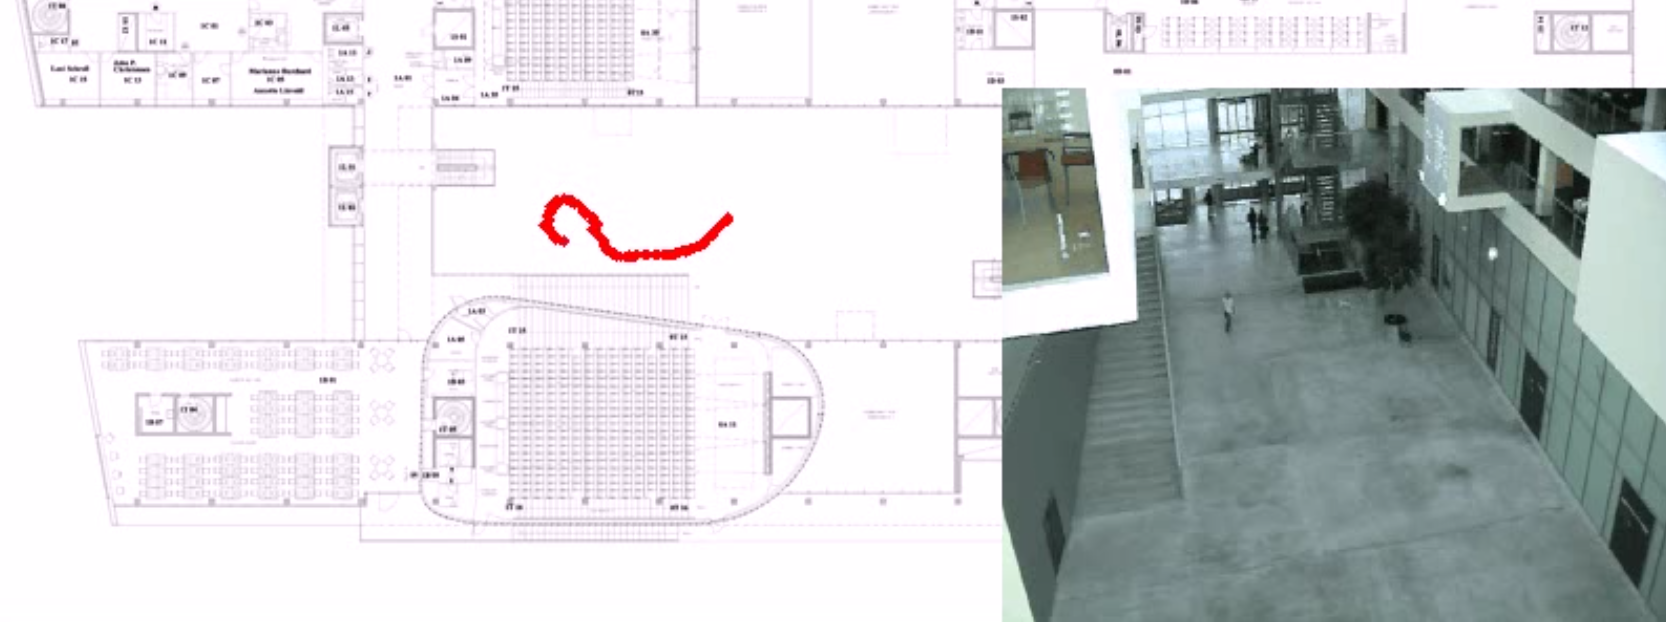
\includegraphics[width=\textwidth]{Handin2/images/personlocationvideo.png}
	\caption{Video Trace}
	\label{fig:video_trace}
\end{figure}

The reason this mapping is useful, is that in the overview map it is easier to see the person's position on the ground plane. On the other hand, depending on the camera angle relative to the ground plane, the accuracy of the estimation can vary depending on the distance from the camera.